\chapter{Related Work}\label{sec:related-work}

\todo[inline]{no section without text}
\section{Foundations}
\todo[inline]{no section without text}

\subsection{Data Visualizations}
Data visualizations is a means of visual communication and have steadily developed since the 16th century~\cite{Friendly2001}.
Otherwise abstract information is visually represented, making complex data more accessible, understandable and usable.
\textcite{Kusinitz2014} explains that the human brain processes visual information 60,000 times faster than text and visual content makes up even 93\% of all human communication.
The purpose of data visualizations is twofold, according to the Interaction Design Foundation: sense-making and communication.
Statistical information is abstract and in data visualization ``we must find a way to give form to that which has none.''~\cite{Few2013}
Successful data visualizations helps the human user to derive knowledge and meta data from the visualization itself, \textcite{Nocke2002} call it ``visual data mining''.

\textbf{Data-driven \dss{}} are applications to support businesses and organizational decision-making activities in which data visualizations play a key part~\cite{Nada2007}~\cite{Poleto2015}.
Visualizations are an obvious choice for managers who demand a quick overview on performance data.
Stephen Few's book ``Show me the numbers'' was named after the phrase often used by sales managers who can't afford to wade through lengthy reports.
\todo[inline]{Prof. Döllner mentioned the emerging ``cockpit'' views}

We can expect to see these technologies more in more in business applications.
\textcite{McAfee2012} from the MIT Center of Digital Business showed that organizations driven most by data-based decision making had 4\% higher productivity rates and 6\% higher profits.
However, little research has been done regarding the performance of \cmvs{} in the field of decision making.
There might be a great potential.
Back in 1997 \textcite{Mayer1997} conducted eight studies to compare the effect of using multimedia on university students.
The studies showed that when using combined visual and verbal explanations the generation of creative problem solutions increased by an average of more than 50\%.

So the application of combined data visualization techniques in decision making seems to be a promising strategy.
Nevertheless is is unclear, which visualization techniques are the most suitable to be used in combination.
If we know what kind of data we are dealing with, what are the best suited visualization techniques?
Let's say we have multidimensional data, is there an order in how people access these multiple dimensions?
How do these visualizations perform and what are best practices to be considered for their implementation?


\subsection{Visual Variables}\label{sec:related-work:visual-variables}
French cartographer Jaques Bertin introduced seven visual varables in 1967~\cite{Bertin2010}.
We can see an example for each in Figure~\ref{fig:related-work:visual-variables}.
These visual variables are used in cartography but can also be applied to data visualization in general.
\textcite{Carpendale2003} explains in detail their use in terms of computational information instead of printed cartography.
\textcite{Garlandini2009} put these visual variables under systematical validation procedures.
The authors conclude that the variable size provides the most accurate and efficent performance while the variable orientation provides the least performance.
\begin{figure}[h!]
  \centering
  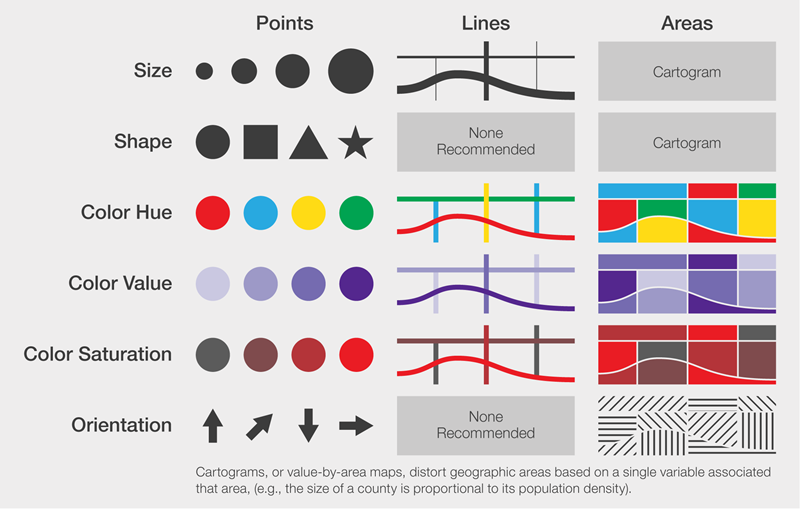
\includegraphics[width=\textwidth]{images/visual-variables.png}
  \caption{Bertin's~\cite{Bertin2010} original visual variables.}\label{fig:related-work:visual-variables}
\end{figure}

\subsection{Treemaps}
The visualization of hierarchical data has a long tradition.
The traditional visual representation of a tree is a directed graph with the root node at the top.
An everyday use case is a directory tree example of a file system, e.g.\ in file browsers or command line utilities like \texttt{tree} in UNIX based operating systems.
As \textcite{Shneiderman1992} mentions, this visualization becomes increasingly large when displaying more than one node and soon exceeds the entire screen size.
\textcite{Johnson1991} proposes the tree map visualization technique, in which each node is a rectangle whose area is proportional to a specified dimension.
Rectangles contain sub-branches of the node as tiles, thereby expressing hierarchy information.
\begin{figure}[h]
    \centering
    \copyrightbox[b]{%
        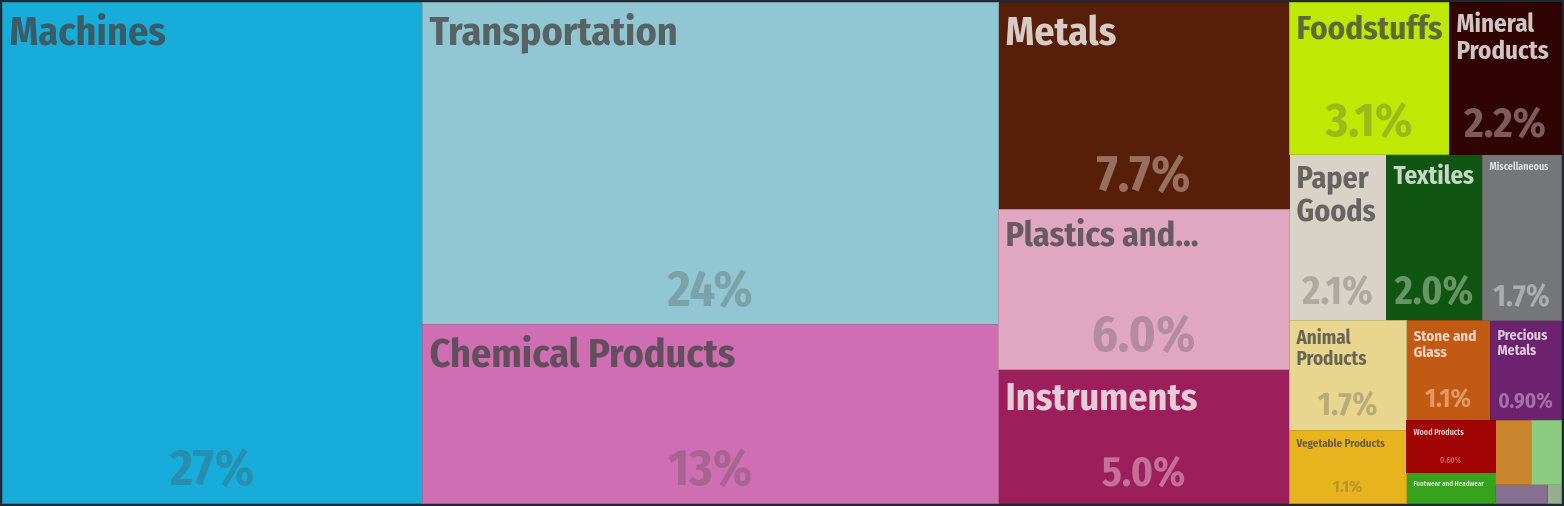
\includegraphics[width=\textwidth]{images/theory/german-exports-1}}{%
        \hfill \ccAttribution{} \ccShareAlike{} Observatory of Economic Complexity~\cite{Macro2017}
    }
    \caption{First hierarchy level of German exports}\label{fig:related-work:treemap-german-exports-1}
\end{figure}

\begin{figure}[h]
    \centering
    \copyrightbox[b]{%
        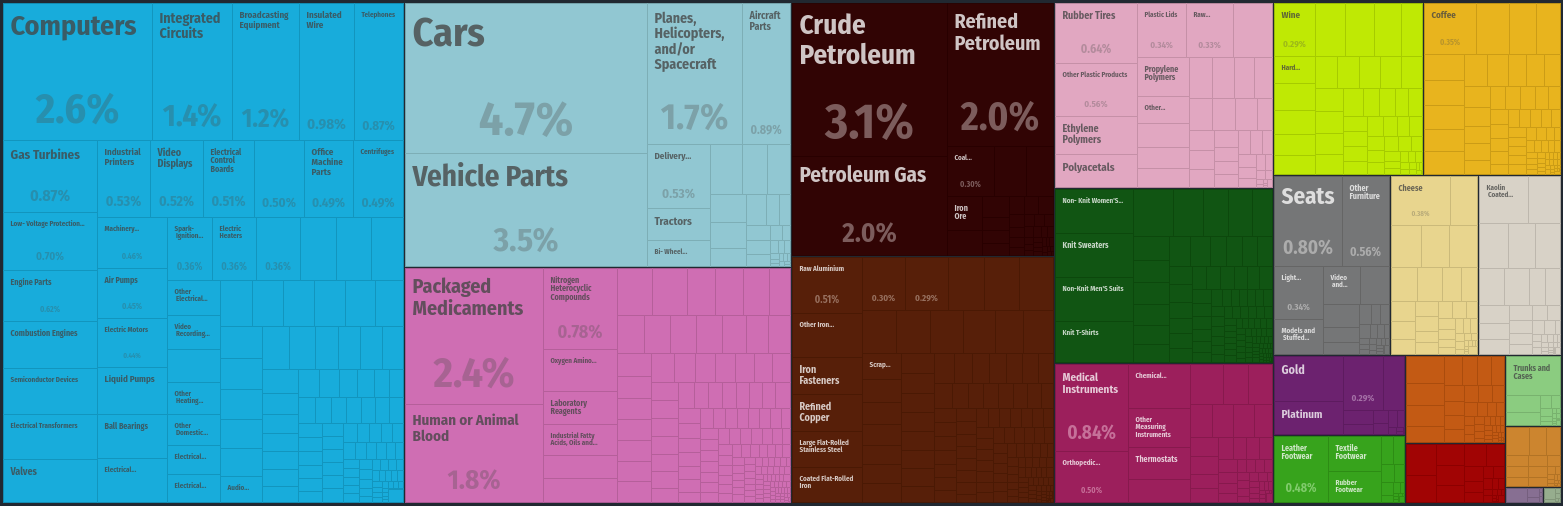
\includegraphics[width=\textwidth]{images/theory/german-exports-2}}{%
        \hfill \ccAttribution{} \ccShareAlike{} Observatory of Economic Complexity~\cite{Macro2017}
    }
    \caption{Second hierarchy level of German exports}\label{fig:related-work:treemap-german-exports-2}
\end{figure}
\todo[inline]{Why is the layout different in the second image?}

We can see an example of an interactive treemap in Figures~\ref{fig:related-work:treemap-german-exports-1} and~\ref{fig:related-work:treemap-german-exports-2}.
German exports are divided in generic groups like ``Machines'' and ``Chemical Products'' and include more specific groups like ``Cars'' and ``Packaged Medicaments''.
The level of hiearchy can be selected with a dropdown menu, so only leaf nodes are displayed at a time.
Treemaps are space-filling visualizations, i.e.\ they make 100\% use of the available screen size.

Note that as the order and placement of the nodes depends on the value of their specified dimension, geographical units of data may may be placed separately on the treemap.

\textbf{\threedTmaps{}} is a concept introduced by \textcite{Bladh2004} in 2004.
The authors transfer the concept of tree maps from two dimensional into three dimensional space.
They introduce StepTree~\cite{Bladh2004}, which is a three dimensional tree map to display a directory layout.
It ``differs from Treemap in that it employs three dimensions by stacking each subdirectory on top of its parent directory.''
3D tree maps are superior to 2D tree maps for tasks with a pronounced topological challenge.
User perform significantly better in interpreting the hierarchical structure.
However, 3D visualizations also introduce some disadvantages as superimposition of objects and a complex view point navigation.

\textbf{\tmap{}} is a term coined by \textcite{Limberger2016}.
A \tmap{} emphasizes physical constraints of a \threedTmap{}, i.e.\ a \tmap{} has all items attached to the ground.
We can see an example of a \tmap{} in figure~\ref{fig:research:ua_treemap}

\begin{figure}[h]
  \centering
  \copyrightbox[b]{%
    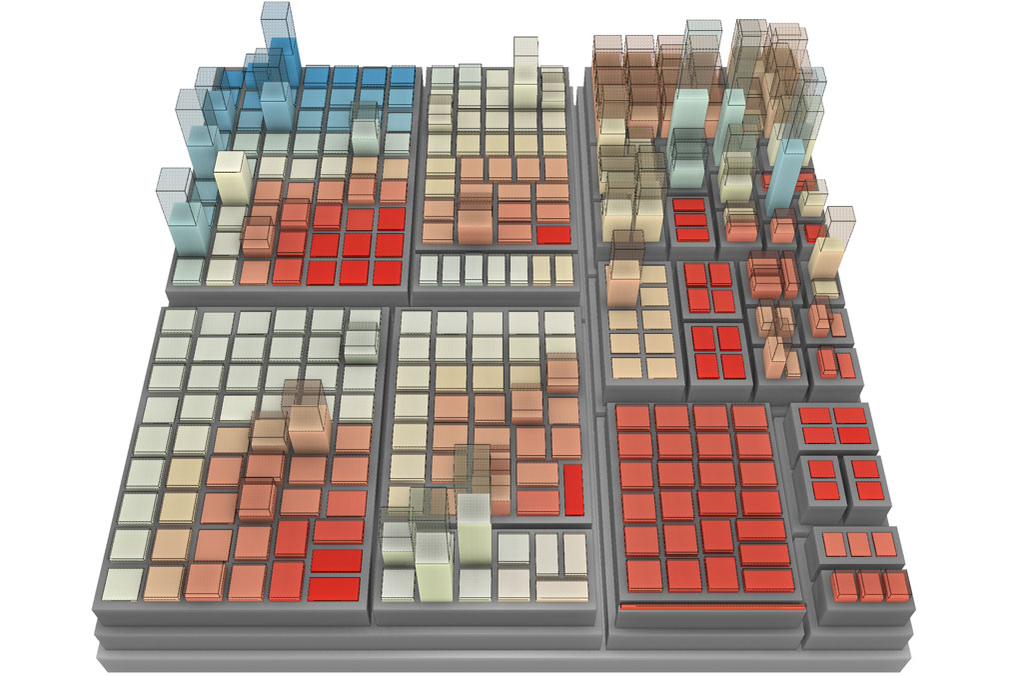
\includegraphics[width=\textwidth]{images/2_5D_treemap_example}}{%
    \hfill \textcopyright{} Hasso-Plattner-Institut\cite{Doellner2017}
  }
  \caption{Example of a \tmap{}}\label{fig:research:ua_treemap}
\end{figure}


\subsection{Geographical Data Visualization}
\todo[inline]{introduction}
\textbf{Flow maps} place stroked lines on top of a geographic map.
They often display the flow of goods or the migration of people.
As we can see in Figure~\ref{fig:related-work:flow-map}, an early example of a flow map is Charles Minard’s depiction of Napoleon’s ill-fated march on Moscow in 1861~\cite{Corbett2001}.
\begin{figure}[h]
  \centering
  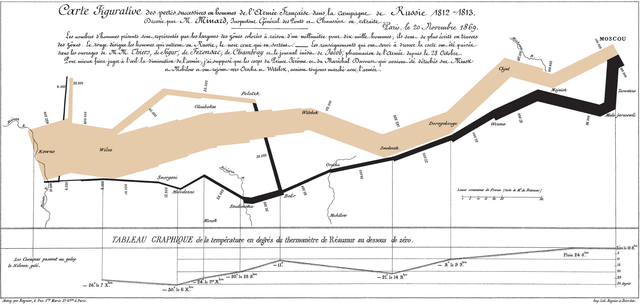
\includegraphics[width=\textwidth]{images/theory/minard}
  \caption{%
    Charles Minard's map of Napoleon's disastrous Russian campaign of 1812.
    Minard managed to represent six values in two graphical dimensions:
    The number of Napoleon's troops, the travelled direction and distance, latitude and longitude relative to specific dates and the temperature.
  }\label{fig:related-work:flow-map}
\end{figure}

\textbf{Choropleth maps} is a thematic map in which areas are shaded or patterned in proportion to the statistical variable being displayed on the map.
A popular use case is the display of population density or per-capita income.
We can see an example of a choropleth map in Figure~\ref{fig:related-work:choropleth}, showing the percentage of obese population in the US\@.
Choropleth maps are widely popular and likely to understand them.
They are very helpful when data is attached to enumeration unites like counties, provinces and countries.

\begin{figure}[h]
  \centering
  \copyrightbox[b]{%
    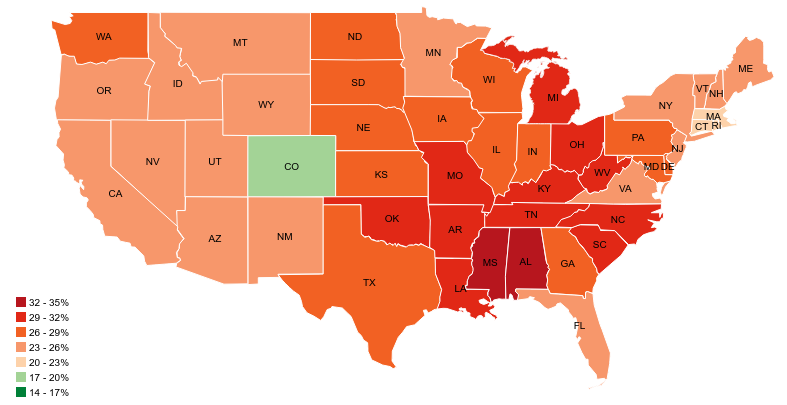
\includegraphics[width=\textwidth]{images/theory/choropleth}}{%
    \hfill National Center for Chronic Disease Prevention and Health Promotion~\cite{NCCDPHP2017}
  }
  \caption{%
    Choropleth Map of Obesity in the United States in 2008.
    Present of population classified as ``obese'' (Body Mass Index in excess of 30), by state.
  }\label{fig:related-work:choropleth}
\end{figure}

\textbf{Graduated Symbol Maps} is a good alternative to a choropleth maps, as it alleviates one of its downsides:
Larger areas may appear more emphasized than smaller ones, thus confounding geographic area with data values.
Instead, symbols are placed over the regions of a map.
As \textcite{Heer2010} point out, these symbols allow for more visal variables to be visualized, i.e.\  symbol size, shape and colour.

\textbf{Cartograms} are used to encode a data attribute in the size of an area.
For this reason geographic regions in cartograms appear distorted.
A common example is to redraw the size of a country based on the the population or gross domestic product of a country.
Area cartograms may be contiguous or noncontiguous, depending on the applied layout algorithm.

\subsection{Coordinated Multiple Views}
According to \textcite{Roberts2007} \cmvs{} is just ``a specific exploratory visualization technique that enables users to explore their data''.
\cmvs{} are characterized by the fact, that they show multiple views side-by-side.
We can see an example in Figure~\ref{fig:research:cmv}.
It displays an on-time performance of airlines, visualized with the ``Crossfilter'' javascript library.
The user can set the borders of an interval with the mouse in each of the views.
The visualization takes the most recent 80 flights from the database that match all given filters.
All visualizations are then updated in real time.
As we can see in the example in Figure~\ref{fig:research:cmv} there seems to be a correlation of a long delay with a later time of the day.

\begin{figure}[h]
  \centering
  \copyrightbox[b]{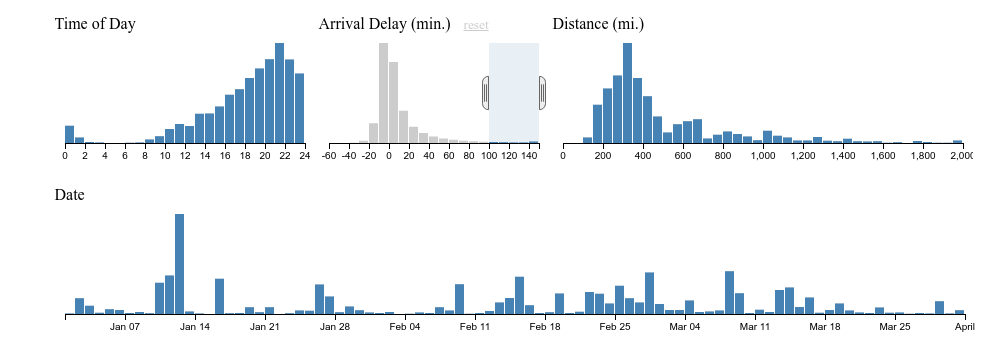
\includegraphics[width=\textwidth]{images/cmv_example}}{\hfill Crossfilter\cite{Bostock2017}}
  \caption{Airline on-time performance: Correlation of time of day with arrival delay. Most recent flight with a delay of more than 100 minutes selected.}\label{fig:research:cmv}
\end{figure}

\textbf{Brushing and Linking}
Most multiple coordinated views also provide some kind of brushing technique.
``The technique of brushing is the principle approach, where elements are selected (and highlighted) in one display, concurrently the same information in any other linked display is also highlighted.''\cite{Roberts2007}

\clearpage
\section{Interaction Theory}\label{sec:interaction-theory}
According to \textcite{Ho2013} interactions are a crucial part of data visualizations, yet most research in the area of data visualization still focuses on visual representations.
Roughly speaking, research on interaction falls into these groups:
How to categorize interaction techniques?
How to find new interaction techniques and apply those to visualizations?

\todo[inline]{Give a rough overview of this section}
\subsection{Interaction Categories}\label{sec:interaction-theory:categories}
\textcite{Shneiderman1996} classifies interactions into these groups:
\begin{enumerate*}[label=(\arabic*)]
  \item
    Gain an \emph{overview} of the entire collection,
  \item
    \emph{zoom} in on items of interest,
  \item
    select an item or group and get \emph{details} when needed,
  \item
    view \emph{relationships} among items,
  \item
    keep a \emph{history} of actions to support undo,
  \item
    allow \emph{extraction} of sub-collections and of the query parameters.
\end{enumerate*}

In 1997 \textcite{Shneiderman1996} classified interactions into these groups:
\begin{enumerate*}[label=(\arabic*)]
  \item
    Gain an \emph{overview} of the entire collection,
  \item
    \emph{zoom} in on items of interest,
  \item
    select an item or group and get \emph{details} when needed,
  \item
    view \emph{relationships} among items,
  \item
    keep a \emph{history} of actions to support undo,
  \item
    allow \emph{extraction} of sub-collections and of the query parameters.
\end{enumerate*}

Two years later, \textcite{Dix1998} identified these categories:
\begin{enumerate*}[label=(\arabic*)]
  \item
    \emph{Highlight and focus} particular subsets of the data,
  \item
    instead of displaying everything simultaneously \emph{access extra information} by drilling down the data,
  \item
    zoom in and out to give an \emph{overview and context},
  \item
    \emph{change parameters} of the \emph{same representation}, e.g.\ another baseline of a stacked bar char,
  \item
    \emph{change representation} of the \emph{same data} by switching the chart type,
  \item
    \emph{link representations} to determine the relationship between items.
\end{enumerate*}

In 2002, \textcite{Keim2002} comes up with the following classification:
\begin{enumerate*}[label=(\arabic*)]
  \item
    Dynamic \emph{projection} to show all combination of data attributes mapped to the axis of a diagram,
  \item
    focus on a smaller subsets by \emph{filtering} out parts of the data,
  \item
    \emph{zoom} into a subset of the data and get a higher level of detail,
  \item
    preserve an overview of the data during drill-down operations is called \emph{distortion}
  \item
    and finally \emph{link and brush} visualizations, to highlight the same data points in multiple visualizations.
\end{enumerate*}

The most recent classification was done in 2007 by \textcite{Yi2007} listing seven categories:
\begin{enumerate*}[label=(\arabic*)]
  \item
    \emph{Select} to mark something as interesting,
  \item
    \emph{explore} to show something else,
  \item
    \emph{reconfigure} to show a different arrangement,
  \item
    \emph{encode} to show a different representation,
  \item
    \emph{abstract/elaborate} show more or less detail,
  \item
    \emph{filter} show something conditionally,
  \item
    \emph{connect} show related items.
\end{enumerate*}

\todo[inline]{The classifications are all redundant! Explain why and choose one classification for later use}
\todo[inline]{Give one example for each category of the chosen classification}

\subsection{Interaction Models}
\todo[inline]{no section without text}

\textbf{Space-Time Cube Operations}
is a concept introduced in 2014 by \textcite{Bach2014} to map temporal data into two dimensional visualizations.
Space-time-cubes are used to model two attributes of continuous data with temporal data along a third axis, therefore the name \emph{cube}.
While the transformations are rather static it is also possible to introduce activity into the transformations.
The authors describe user-independent \emph{animations} and user-controlled \emph{interactions}.
E.g.\ a transformation may display a given slice of the cube.
An animation would display one slice at a time and display the next slice every second.
Whereas the interaction would show the slice determined by a user-controlled slider.
Various transformations and their best use in practice are evaluated in this work.
The work focuses on temporal data and otherwise continuous data.
Interactions are not seen as an abstract entity, that need to be agnostic of the underlying data structure and visualization.
The authors admit ``our framework does not provide much guidance for interaction design: the design space for interactive operations has only been partially explored.''\cite[Other limitations, p.~15]{Bach2014}

\textbf{ITlib\cite{Figueroa2001}} is an architecture and a framework of interaction techniques for virtual reality applications, designed to be extensible and flexible.
New interaction techniques can easily be added and application specific code is seamlessly integrated.
On a low level an interaction technique ``is modeled as a set of filters connected in a small data flow''\cite[Basic concept, p.~2]{Figueroa2001}.
These filters are the smallest process unit in the data flow.
Composed of input and output ports, they communicate with other filters, to receive data input from predecessors and send data output to successors.
The framework specifies and stores the interaction techniques along with its filters, the execution model and the scene in XML documents.
The authors chose XML because it can be parsed easily and they generate code in order to target various virtual reality toolkits and environments.

Even though the system describes interactions in an abstract way, the domain of the framework is clearly the interaction of a human body within a 3D virtual reality.
Certain assumptions are made, including the data model, which is the 3D scene, and human computer interaction devices, like the user's hand or the user's head.
The goal is not to better understand the data, as the data model in this case is the 3D scene, and not statistical data.
Most important, the framework describes interaction techniques for a single viewpoint but not for coordinated multiple views.

\textbf{Focus+Context Visualization} by \textcite{Bjork1999} is one of the few formalizations of information visualizations.
The authors describe this formalization based on first-level and second-level visualization:
\subparagraph{Visualizations} referred to as $IV$, are triples of a set $[D]$ of underlying data, a visual representation $V$ and $I$ which is the possible interaction or manipulation.
\begin{equation}
  IV([D], V, I)
\end{equation}
If $I$ affects $[D]$ we can manipulate the underlying data set.
Examples would be changes in a spreadsheet editor, or a change of the start and end date of an appointment in a calendar.
When $V$ is affected by $I$ the user can manipulate $IV$ in order to change the way $[D]$ is represented, e.g.\ choosing a different level of detail as shown in Figures~\ref{fig:related-work:treemap-german-exports-1} and~\ref{fig:related-work:treemap-german-exports-2}.

\subparagraph{Second-level Visualizations} are information visualizations consecutively applied.
The underlying data set $[D]$ of the previous formula is replaced with some information visualization $IV$, which is compatible with $IV'$.
\begin{equation}
  IV'(IV, V', I')
\end{equation}


Focus+context visualizations are second-level visualizations.
An example given by the authors is the  ``rubbersheet'' visualization, that visually distorts a first-level visualization similar to a magnifier.

